%=============================================================== %	
	\begin{figure}


\includegraphics[width=0.5\linewidth]{cythonlogo}

\end{figure}

\begin{figure}
\centering
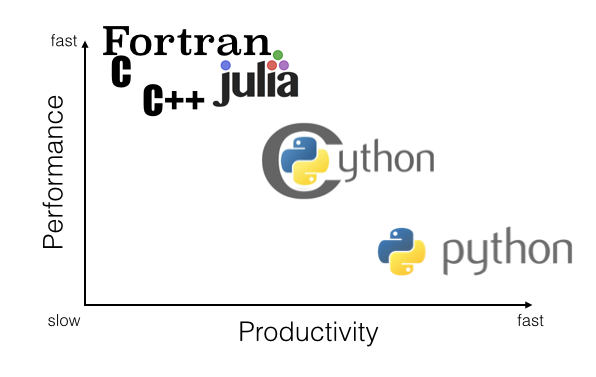
\includegraphics[width=0.7\linewidth]{cython_vs_chart}

\end{figure}

\end{frame}
%===========================================================%
\begin{frame}
	
	\large
\frametitle{Performance Modules : Cython and Numba}
A number of modules are available to help with performance. These include Cython and Numba.

\begin{description}
	\item[Cython] Cython
	is a Python module which facilitates using a simple Python-derived creole to write functions that can be
	compiled to native (C code) Python extensions. 
	
	
	\item[Numba] 
	Numba uses a method of just-in-time compilation to
	translate a subset of Python to native code using \textit{Low-Level Virtual Machine} (LLVM).
\end{description} 

\end{frame}
%=========================================================== %
\begin{frame}
	\begin{figure}
\centering
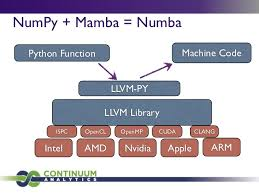
\includegraphics[width=0.99\linewidth]{numba}

\end{figure}